\documentclass[twocolumn]{IEEEtran}
\usepackage[utf8x]{inputenc}
\usepackage{amssymb,amsfonts}
\usepackage[tbtags]{amsmath}
\usepackage{graphicx}
\usepackage{cite}
\usepackage{slashbox}
\usepackage{pict2e}
\usepackage{float}
\usepackage[all]{xy}
\usepackage{graphics,graphicx,color,colortbl}
\usepackage{times}
\usepackage{subfigure}
\usepackage{wrapfig}
\usepackage{multicol}
\usepackage{cite}
\usepackage{url}
\usepackage[tbtags]{amsmath}
\usepackage{amsmath,amssymb,amsfonts,amsbsy}
\usepackage{bm}
\usepackage{algorithm}
\usepackage{algorithmic}
\usepackage[centerlast, small]{caption}
\usepackage[colorlinks=true, citecolor=blue, linkcolor=blue, urlcolor=blue, breaklinks=true]{hyperref}
\begin{document}
\title{Práctica Integradora}
\author{José Fabio Lozano Ovalle Código: $222982$\\
	Wilson Orlando Macias Fuquen Código: $223101$\\
	David Ricardo Martínez Hernández Código: $261931$}
\maketitle
\markboth{Universidad Nacional de Colombia}{}
\floatname{algorithm}{Algoritmo}
\begin{abstract}
 Se diseñara un circuito el cual informara el sobrecalentamiento de las piezas de una cortadora, dicho circuito constara de un termistor, el cual activara un sistema de réles acoplados a un circuito $RC$ activando la alarma de sobrecalentamiento después de $1$ minuto de continua exposición. Obteniendo un sistema de protección eficaz para la maquina cortadora.
\end{abstract}

\section{Objetivos}
\begin{itemize}
 \item Utilizar los conocimientos adquiridos a lo largo del curso para resolver un problema práctico de ingeniería.
 \item Caracterizar los elementos a utilizar en el diseño del sistema de protección (Réles y termistores).
\end{itemize}

\section{Introducción}
\noindent
Cuando una maquina esta expuesta constantemente a temperaturas elevadas su vida útil se reducirá debido al desgaste térmico, y en el caso particular de una cortadora se hace más evidente ya que sus piezas son elementos de precisión y al estar en contacto con altas temperaturas reducirá su tiempo de vida.\\
El conocimiento a adquirido a lo largo del curso nos da herramientas para proporcionar una solución a este problema de ingeniería.

\section{Marco Teórico}
\subsection{Réle}
\noindent
El relé está formado por un contacto móvil o polo y un contacto fijo, como interruptor. Pero también hay relés que funcionan como un conmutador, porque disponen de un polo (contacto móvil) y dos contactos fijos Fig. \ref{fig1}
\begin{figure}[H]
	\centering
		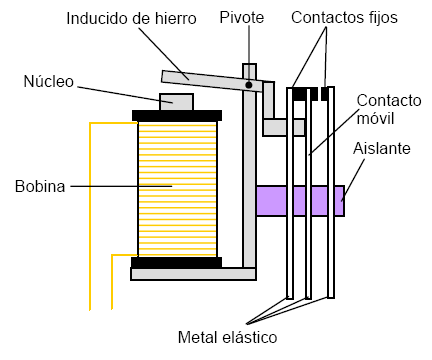
\includegraphics[scale=0.5]{rele.png}
	\caption{Esquema de un relé}
	\label{fig1}
\end{figure} 
\noindent
Cuando no pasa corriente por la bobina el contacto móvil está tocando a uno de los contactos fijos (en la Fig. \ref{fig1} el de la izquierda). En el momento que pasa corriente por la bobina, el núcleo atrae al inducido, el cual empuja al contacto móvil hasta que toca al otro contacto fijo (el de la derecha). Por tanto, funciona como un conmutador.

\subsection{Zumbador}
\noindent
El zumbador es un aparato cuyo funcionamiento se basa en el electroimán. Cuando cerramos su circuito haciendo que llegue corriente eléctrica al electroimán, éste atrae a la armadura azul, que golpea a chapa superior (gris) que está unida a uno de los polos del electroimán, produciendo un ruido. Al mismo tiempo, se separa del tornillo de ajuste, abriéndose así el circuito e impidiendo la llegada de corriente eléctrica al electroimán. La armadura, que ya no es atraída por el electroimán, retrocede y se pone en contacto de nuevo con el tornillo de ajuste, cerrándose otra vez el circuito. Este proceso se repite ininterrumpidamente mientras mantengamos alimentado el zumbador.

\subsection{Termistores}
\noindent
Los Termistores son resistores térmicamente sensibles, existen dos tipos según la variación de la resistencia/coeficiente de temperatura, pueden ser negativos (NTC) o positivos (PTC).
Son fabricados a partir de los óxidos de metales de transición (manganeso, cobalto, cobre y níquel) los termistores NTC  son semiconductores dependientes de la temperatura. Operan en un rango de $-200º C a + 1000° C$. Un NTC debe elegirse cuando es necesario un cambio continuo de la resistencia en una amplia gama de temperaturas. Ofrecen estabilidad mecánica,  térmica y eléctrica, junto con un alto grado de sensibilidad.\\
La excelente combinación de precio y el rendimiento ha dado lugar a una amplia utilización de los NTCs en aplicaciones  tales como medición y control de temperatura, compensación de temperatura y medición del flujo de fluidos.

\section{Hipótesis}
\noindent
Se desea obtener un circuito con un sistema de reacción a temperatura, es decir que a una temperatura ambiente el circuito no reaccione y la alarma de advertencia permanezca apagada, cuando al temperatura se aumente a un valor con el cual los elementos de la maquina estén en peligro, el circuito reaccione y la alarma se encienda al rededor de un minuto luego de llegar a esta temperatura critica.

\section{Materiales}
\begin{itemize}
 \item Alambres
 \item Condensadores
 \item Inductancias
 \item Resistencias
 \item Termistores
 \item Zumbador
\end{itemize}

\section{Montaje a realizar}
\noindent
Para este montaje los valores de las resistencias, el condensador y fuente, se obtendrán después de caracterizar el termistor y el réle, para poder obtener el tiempo de reacción deseado.
\begin{figure}[H]
	\centering
		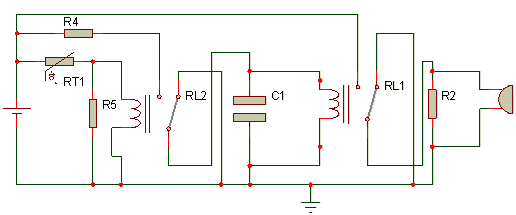
\includegraphics[scale=1]{montaje.png}
	\caption{Esquema del montaje}
	\label{fig2}
\end{figure} 

\bibliographystyle{ieeetran}
\begin{thebibliography}{99}
\bibitem{sadiku} Alexander, Charles K. \&  Sadiku, Matthew N.O.
{\em ```Fundamentals of Electric Circuits"'}.
McGRAW-HILL, ISE Editions, 1999.

\bibitem{dorf} Dorf  \& Svoboda.
{\em ```Circuitos Eléctricos"'}.
Alfaomega, Sexta Edición, 2006.

\bibitem{hayt} Hayt, William H. Jr., Kemmerly, Jack E. \& Durbin, Steven M.
{\em ```Análisis de circuitos en ingeniería"'}.
McGRAW-HILL, Séptima Edición, 2007.

\bibitem{nahvi} Nahvi, Mahmood \& Edminister, Joseph A.
{\em ```Theory and Problems of Electric Circuits"'}.
McGRAW-HILL, Fourth Edition, 2003.

\end{thebibliography}
\end{document}